\documentclass{beamer}
\usepackage{graphicx}
\usepackage{ulem}

\title{Lessons Learned in Spike Sorting: The \ensuremath{n=1} Perspective}
\author{Eddie Yan}
\date{June 21, 2013}

\begin{document}
    \begin{frame}
        \titlepage
    \end{frame}

    \begin{frame}{What I did}
            \pause
        \begin{itemize}
            \item October 2012--November 2012: Changing parameters
(\texttt{allcluststdev}) and doing unit quality by hand
            \pause
            \item November 2012--December 2012: Automatic unit quality via SNR
            \pause
            \item January 2013: Changing \texttt{mergeclusterstdev}
            \pause
            \item January 2013--February 2013: Trying to optimize
            \pause
            \item March 2013--June 2013: Improving merge deliberation
        \end{itemize} 
    \end{frame}

    \begin{frame}{Changing \texttt{allcluststdev} (Mouse 5 Jun14a)}
        \begin{itemize}
            \pause
            \item It doesn't seem to affect the quality of units produced at the
end of sorting, at least with the range of parameters tried \ensuremath{\{6,7,8,9
,10\}}       
            \pause
            \item Doing unit quality by hand on the same dataset again and again
is tedious and prone to inconsistency
        \end{itemize}
    \end{frame}
    
    \begin{frame}{This Figure is Really Old (Mouse 5 Jun14a)}
        \begin{center}
            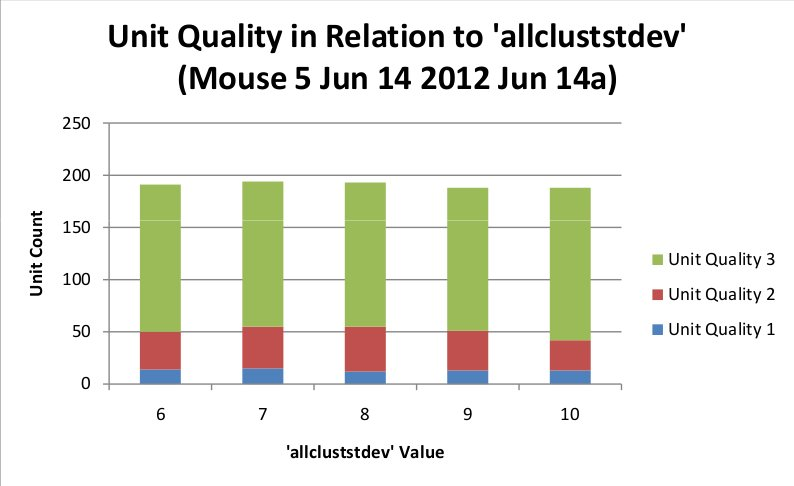
\includegraphics[width=110mm]{images/allcluststdev.jpg}
        \end{center}
    \end{frame} 

    \begin{frame}{Auto-Unit Quality/Semi-automatic Unit Quality}
        \begin{itemize}
            \pause
            \item Doing unit quality by hand was extremely inconsistent and
unreliable
            \pause
            \item Find a metric to allow computers to do it automagically!
            \pause
            \item What worked? SNR!
            \pause
                \begin{itemize}
                    \item Sort of
                \end{itemize}
            \end{itemize}
    \end{frame}
    
    \begin{frame}{Auto-Unit Quality/Semi-automatic Unit Quality and Quasi-SNR}
        \textbf{Steps: }
        \begin{enumerate}
            \item Interpret spikes at face value: a series of voltages in
discrete time
            \pause
            \item Compute their root-mean-square (RMS) power
            \pause
            \ensuremath{\sqrt{\frac{1}{n}\left(x^2_1 + x^2_2 + ... +
x^2_n\right)}}
            \pause
            \item Why is it quasi-SNR? We treat the mean as the ``signal'' and
simply subtract it from each of the spikes to get the ``noise''
            \pause
            \item Get the signal to noise ratio
            \pause
            \item Decide unit quality
            \begin{itemize}
                \item We can choose percentiles, further qualifiers, etc.
                \pause
                \item Qualifier that works well: restricting consideration to
points near the peak of the spike
            \end{itemize}
        \end{enumerate}
    \end{frame}

    \begin{frame}{Pitfalls in Auto-Unit Quality}
        \begin{itemize}
            \pause
            \item Even with only 3 grades of unit quality, the number of
empirically derived parameters grows quickly
            \pause
            \item The process can be confused by high-SNR artifacts/non-units
that would be caught by a human
            \pause
            \item Best use case for auto-unit quality?
            \begin{itemize}
            \pause
                \item Consistent scoring of different sorting algorithms
            \end{itemize}
        \end{itemize}
    \end{frame}

    \begin{frame}{Changing \texttt{mergecluststdev (Mouse 5 Jun14a)}}
        \begin{center}
        \begin{tabular}{l c c c r}
        \pause
        \texttt{mergecluststdev}&1&2&3\\
        \pause
        Unit Quality 1&45&43&40\\
        \pause
        Unit Quality 2&139&148&146\\
        \pause
        Unit Quality 3&103&104&106\\
        \pause
        Total&287&295&292\\
        \pause
        Merges in \texttt{get\_penultimate}&260&61&24
        \end{tabular} 
        \end{center}
        \begin{itemize}
            \pause
            \item Observations
            \begin{itemize}
                \item \texttt{get\_penultimate} merges are usually not very
significant
                \item bulk of merges are done in \texttt{get\_final\_units}
            \end{itemize}
        \end{itemize}
    \end{frame}

    \begin{frame}{Applying lessons learned with \texttt{mergecluststdev}: merges
in \texttt{get\_final\_units}}
    \begin{itemize}
        \pause
        \item Goal is to improve merges in \texttt{get\_final\_units}
        \pause
        \item Techniques tried:
        \begin{enumerate}
            \pause
            \item \sout{Mahalanobis Distance}
            \item {Principal Component Analysis}
        \end{enumerate}
     \end{itemize}
    \end{frame} 
    
    \begin{frame}{Principal Component Analysis in One Slide}
        \begin{itemize}
            \pause
            \item \textbf{Motivation}: Units are messy to compare, as spikes
each have \ensuremath{\approx} 47 sampled points of amplitude
            \pause
            \item Principal component analysis (PCA) allows us to transform each
spike into 47 data points of decreasing significance, so a comparing e.g. only
the first three dimensions becomes reasonable (we go from
\ensuremath{\mathbb{R}^{47}} to \ensuremath{\mathbb{R}^3})
         \end{itemize}
    \end{frame}
     
    \begin{frame}{How PCA Was Used in Sorting}
        \begin{itemize}
            \pause
            \item Used in \texttt{get\_final\_units} as an alternative to the
current Euclidean-distance based merge process
            \pause
            \item For each unit \textbf{\emph{i}}:
            \begin{enumerate}
                \pause
                \item Consider each PCA-transformed spike in
\ensuremath{\mathbb{R}^3} space
                \item Form a cluster of points corresponding to the spikes of that unit in
\ensuremath{\mathbb{R}^3}
                \pause
                \item Compare this unit with every other unit
                \pause
                \item For the other unit \textbf{\emph{j}}, also form 
cluster of points corresponding to spikes in \ensuremath{\mathbb{R}^3}
                \pause
                \item Consider the distance between the clusters to decide if
the two units should be merged (the smaller the distance between the clusters of
two units, the more likely they should be merge)
            \end{enumerate}
         \end{itemize}
    \end{frame}

    \begin{frame}{Problems Encountered with PCA and Their Attempted Solutions}
        \begin{itemize}
            \pause
            \item The PCA merge process is not inherently scale-invariant
            \begin{itemize}
                \pause
                \item Normalize the data using z-scores
            \end{itemize}
                \pause
            \item The PCA merge process is more sensitive to ``garbage units''
than the old Euclidean-distance based merge process
            \begin{itemize}
                \pause
                \item Use intensive
garbage-discarding/``sanity-checks''---\texttt{get\_sane} before the merge
process
            \end{itemize}
        \end{itemize}
    \end{frame}
\end{document}
